\documentclass{article}[12pt]
\renewcommand{\baselinestretch}{1.5}

\usepackage[parfill]{parskip}
\usepackage[affil-it]{authblk}
\usepackage[space]{grffile}

\usepackage[a4paper]{geometry}
\geometry{verbose}
\usepackage{float}
\usepackage{graphicx}
\usepackage{setspace}
\usepackage{caption}

\usepackage[utf8]{inputenc}
\usepackage[english]{babel}

\usepackage{latexsym,textcomp,longtable,tabulary}
\usepackage{booktabs,array,multirow}
\usepackage{amsfonts,amsmath,amssymb,mathbbol,calc}
\usepackage{subfigure,color,blindtext,enumitem,siunitx}

\usepackage{mathtools}
\usepackage{url,hyperref,etoolbox}
\numberwithin{equation}{section}
\hypersetup{colorlinks=false,pdfborder={0 0 0}}

%+figure layout options
\restylefloat{figure}
\setlist{leftmargin=*,before=\setlength{\rightmargin}{\leftmargin}}
%-figure layout options

\providecommand\citet{\cite}
\providecommand\citep{\cite}
\providecommand\citealt{\cite}

\setlength{\parskip}{1em}
\makeatletter
\makeatother


\newif\iflatexml\latexmlfalse
\providecommand{\tightlist}{\setlength{\itemsep}{0pt}\setlength{\parskip}{0pt}}%
\AtBeginDocument{\DeclareGraphicsExtensions{.pdf,.PDF,.eps,.EPS,.png,.PNG,.tif,.TIF,.jpg,.JPG,.jpeg,.JPEG}}
\begin{document}

\title{
On the affect of the Laplacian in equlibration\\
dynamics of the Spherical Model
}

\author{Gregory Szep}
\affil{King's College London}
\date{\today}
\maketitle

\section{Mathematical Analysis}
\vspace{-10pt}
\subsection{Motivation for the Model}
Consider $N$ nodes in a undirected network passing around a finite resource.
Eventually the resource will equilibrate within the network solely due it its
finiteness. We wish to study the equilibration timescales of such a problem,
where finiteness of the resource and connectedness of the network may be
expressed is a variety of ways, giving rise different flavours of the
Sherrington-Kirkpatrick spherical model.

Exact dynamical solutions can be obtained if finiteness of the resource
is the expressed as a constant $L_2$ norm across all the nodes. In addition,
if the connectedness of the network is known, it may be used to obtain explicit
expressions --- at least in some limit --- for the dynamics of the resource,
and hence timescales can be extracted.

The Wigner ensemble is used to generate the connectivity in an attempt to
minimise a priori assumptions on it. Then intorducing the $M$-dimensional
periodic lattice laplacian allows the study of the model as it departs from
randomness and gains spatial structure. Is it possible to extract the dimension
of the manifold that the nodes lie on simply from observed correlations and
equilibration timescales in the resource? This work may have applications in
dimensionality reduction methods.

\subsection{Spherical Sherrington-Kirkpatrick Model}
Let the resource across $N$ nodes be represented by vector $s(t)\in\mathbb{R}^N$,
and the weighted undirected connections between them be a Hermitian $N\times N$ matrix
$\mathbf{J}$. This matrix represents the rate at which the resource is passed between
nodes. Without finiteness, we can solve the linear equations, revealing that
the resource at different nodes would diverge or go to zero depending on the sign
of the eigenvalues of $\mathbf{J}$. This does not seem reasonable.

Therefore a lagrange multiplier $\mu(t)\in\mathbb{R}$ is introduced which holds
the $L_2$ norm of vector $s(t)$ constant. This implicitly introduces a nonlinearity.
The dynamics is cast as a Langevin Equation with white noise $\xi(t)\in\mathbb{R}^N$
which is characterised by its moments $\langle\dots\rangle$. Eventually the resource
will equilibrate due it its finiteness, subject to the amplitude of the noise.
The symbol $\mathbb{1}$ represents the diagonal identity.
\begin{align}
  \partial_t s = \big[\mathbf{J}-\mathbb{1}\mu(t)\big]s+\xi
\end{align}
\vspace{-40pt}
\begin{align}
  \left\langle\xi(t)\right\rangle=\mathbb{0}\qquad
  \left\langle\xi(t)\xi(t')\right\rangle=2T\mathbb{1}\delta(t-t')
\end{align}
\vspace{-40pt}
\begin{align}
\text{where}\quad\mu(t) = \frac{1}{N}s^{\top}\left(\mathbf{J}s+\xi\right)
\quad\text{enforces constraint}\quad s^\top\! s=N
\label{eq:constraint}
\end{align}
\subsubsection{Dynamical Properties}
It is possible to solve the inhomogenous time-dependent ordinary linear system of
differential equations for $s(t)$ using integrating factor method and rotate
into the eigenbasis $\sigma_{\lambda}(t)\in\mathbb{R}$ of matrix $\mathbf{J}$. This does not
yield a closed form for $\mu(t)$ however. Following the derivation by Cugliandolo, L. F.
and Dean D. S.~\cite{} yields the moments explicitly for the uniform
initial condition $\sigma_{\lambda}(0)=1$. Here the complexity lies in performing
the inverse laplace transform $\mathcal{L}^{-1}$ which in turn depends on the
eigenvalue distribution $p(\lambda\in\mathbf{J})$.
\begin{align}
  \begin{matrix}
  \langle \sigma_{\lambda}(t)\rangle=
    \frac{\mathbb{e}^{\lambda t}}{\sqrt{\Gamma(t)}}
    &&\qquad
  \begin{matrix}
  \langle s(t)^{\top}\!\!s(t')\rangle=
  \frac{N}{\sqrt{\Gamma(t)\Gamma(t')}}
  \bigg(
  \int_{\mathbb{R}} p(\lambda\in\mathbf{J})\mathbb{e}^{\lambda(t+t')}\mathrm{d}\lambda
  \\+2T
  \int_{\mathbb{R}}p(\lambda\in\mathbf{J})\int_{0}^{\min(t,t')}\!
  \Gamma(\tau)\mathbb{e}^{\lambda(t+t'-2\tau)}
  \mathrm{d}\tau\mathrm{d}\lambda
  \bigg)
  \end{matrix}
  \label{eq:moments}
  \end{matrix}
\end{align}
\vspace{-20pt}
\begin{align}
  \Gamma(t)=
    \sum_{k=0}^{\infty}(2T)^k
    \mathcal{L}^{-1}\left[\Phi(s)^k\right]\quad\text{where}
    \quad
    \Phi(s)=\int_{\mathbb{R}}\frac{p(\lambda\in\mathbf{J})}{s-2\lambda}\mathrm{d}\lambda
    \label{eq:gamma}
\end{align}
\subsubsection{Equilibrium Properties}
If the Langevin dynamics can be written as the gradient of some potential $V(s)$
then the steady state is distrubted according to a Gibbs measure of inverse
temperature $\beta$ with partition function $Z_N(\beta)$.
Indeed it is possible to write down $V(s)$ without the constraint enforced by
$\mu(t)$; instead it is included via a static lagrange multiplier $\mu$ with
an average self-consistency condition.
\begin{align}
  Z_N(\beta)=\int_{\mathbb{R}^N}\!\mathbb{e}^{-\beta V(s)-\mu\,s^{\top}\!s}\,\mathrm{d}s
  \qquad\text{where}\quad
  \left\langle s^\top\!s\right\rangle=-\partial_\mu\ln Z_N(\beta)
  \qquad
  V(s)=-\frac{1}{2}s^{\top}\mathbf{J}s
\end{align}
Rotating into the eigenbasis $\sigma_\lambda$ leaves the integral invariant and
allows factorisation
\begin{align}
  Z_N(\beta)
  &= \prod_{\lambda\in\mathbf{J}}
    \int_{\mathbb{R}}
      \mathbb{e}^{-(\mu-\frac{\lambda\beta}{2})\sigma_\lambda^2}
    \,\mathrm{d}\sigma_\lambda \\
  &= \mathbb{e}^{-\frac{1}{2}\sum_{\lambda\in\mathbf{J}}\ln\left(\frac{\mu-\lambda\beta/2}{\pi}\right)}
  \qquad\mu>\frac{\Lambda\beta}{2}
  \quad\text{where}\quad
  \Lambda=\max_{\lambda\in\mathbf{J}}\{\lambda\}
\end{align}
The average self-consistency condition $\left\langle s^\top\!s\right\rangle=N$ for
solves for $\mu$ with an integral over the density $p(\lambda\in\mathbf{J})$.
For high temperatures $\beta\searrow 0$ the singularity in the integrand
$\lambda^*\nearrow\infty$ moves out of the bounds of support of
$p(\lambda\in\mathbf{J})$, which suggests that the occupation of modes $\lambda$
at equilibrium is given only by the eigenvalue distirbution. As the temperature
approaches $\beta\nearrow 2\mu/\Lambda$ the singularity reaches the upper
bound of the density $\lambda^*\searrow\Lambda$. At this critical value the
singularity weights the mode $\lambda^*$ macroscopically. This phase transition
has the flavour of Bose condensation.
\begin{align}
  \left\langle s^\top\!s\right\rangle
  =\frac{N}{\beta}\int_{\mathbb{R}}\frac{p(\lambda\in\mathbf{J})}{\frac{2\mu}{\beta}-\lambda}\,\mathrm{d}\lambda
\end{align}
From this it is possible to determine the occupation at any given mode $\lambda$
which is the same as the moment $\langle \sigma_{\lambda}(t)\rangle$ in the
infinite time limit.
\begin{align}
  \lim_{t\rightarrow\infty}\langle \sigma_{\lambda}(t)\rangle
  =N^{1/2}\sqrt{1-\frac{1}{\beta}\int_{\mathbb{R}}
  \frac{p(\lambda'\in\mathbf{J})}{\lambda-\lambda'}\,\mathrm{d}\lambda'}
  \label{eq:equilibrium}
\end{align}
\pagebreak
\subsection{Hermitian Wigner Ensemble}
Suppose the connections between nodes are given by a random matrix
$\mathbf{H}$ taken from the Hermitian Wigner ensemble, whos upper triangle elements
$[\mathbf{H}]_{ij}$ are distributed according to a density $\mathbb{P}$ with
subexponential tails~\cite{} with expectation $\mathbb{E}$ and variance
$\mathbb{V}$, such that in the limit $N\rightarrow\infty$ the eigenvalue
spectrum converges to the semicircle law $p(\lambda\in\mathbf{H})\rightarrow\cap(\lambda|J)$.
Below the symbols $\mathbf{0}$ and $\mathbf{1}$ denote constant matrices of zeros and ones
respectively.
\begin{figure}[H]
\centering{}
\captionsetup{justification=centering}
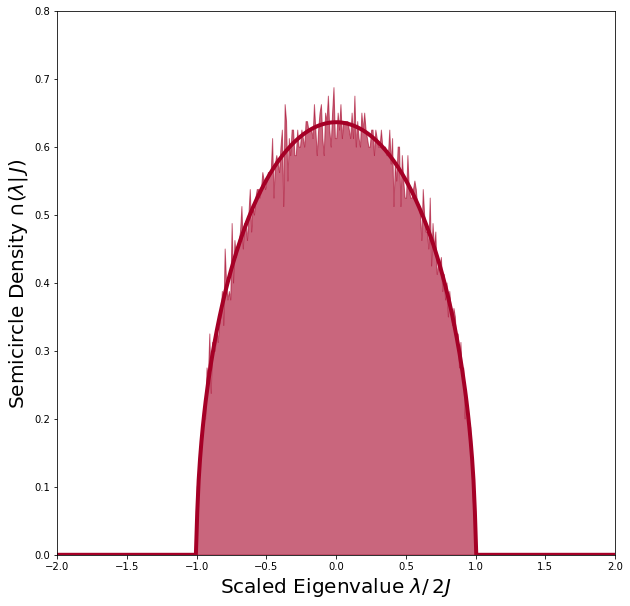
\includegraphics[scale=0.4]{figures/semicircle}
\caption{Empirical histogram of wigner ensemble eigenvalues and analytical semicircle
distribution $\cap(\lambda|J)$, demonstrating the corresponance of the law in the
$N\rightarrow\infty$ limit}
\label{fig:semicircle}
\end{figure}
\vspace{-45pt}
\begin{align}
\cap(\lambda|J)=\frac{\Pi(\lambda/2J)}{2\pi J^2}\sqrt{4J^2-\lambda^2}\label{eq:semicircle}
\quad\quad
    \Pi(x)=
      \begin{cases}
        1 & |x|<1\\
        0 & |x|\geq1\\
      \end{cases}\\
\mathbb{E}[\mathbf{H}]=\mathbf{0}
\quad
\mathbb{V}[\mathbf{H}]=\frac{J^2}{N}(\mathbf{1}+\mathbb{1})
\quad\qquad\qquad\\
\mathbb{P}\left(
t^\alpha\leq
\left|[\mathbf{H}]_{ij}\right|
\right)\leq e^{-t}
\quad
\forall t\geq\alpha,\forall i,j
\quad\qquad\quad
\end{align}
The Heaviside Pi function $\Pi(x)$ bounds the distirbution. Note
the requirement on the distribution of the elements $[\mathbf{H}]_{ij}$
is quite general and allows for the choice of a sparse random matrix. This is
useful when optimising the numerical integration of the equations of motion; in
particular sparse memory access allows for efficient implementation on graphics
processing units~\cite{}.

If the spherical model has completely random interations the semicircle
distribution \eqref{eq:semicircle} can be integrated in to obtain $\Phi(s)$.
To match the terms of the expansion for $\Gamma(t)$ to known inverse laplace
transforms some algebraic trickery is required: the infinite sum is evaluated first.
Then the result is expanded in terms the denominator part that is a function of $s$.
Only then do the terms match the laplace transforms of modified Bessel functions
of the first kind $\frac{I_{l}(4Jt)}{t}$. These have well-known asymtotics for
$t\rightarrow\infty$. Finally the moments \eqref{eq:moments} can be numerically
evaluated as shown in Figure \ref{fig:wigner}.
\begin{figure}[H]
\centering{}
\captionsetup{justification=centering}
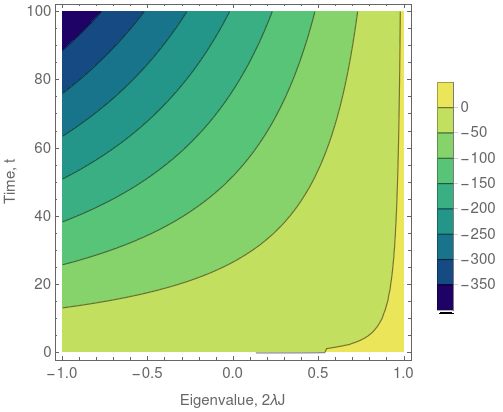
\includegraphics[scale=0.4]{figures/wigner}
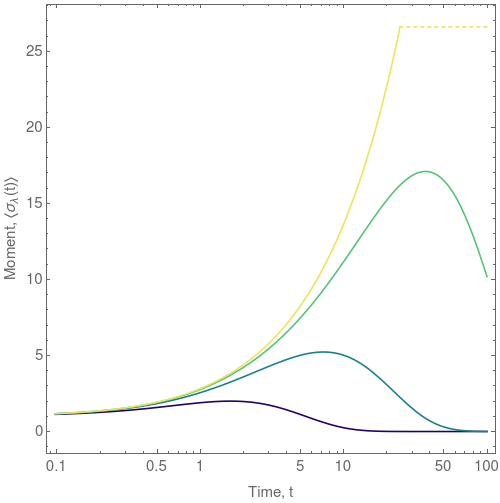
\includegraphics[scale=0.33]{figures/wigner1}
\caption{Moments $\langle \sigma_{\lambda}(t)\rangle$
in the $\lambda,t$ eigenvalue time plane for a given temperature $T<J$. The contours are on a log
scale, revealing that only the maximal eigenvalue component does not decay to zero}
\label{fig:wigner}
\end{figure}
\vspace{-30pt}
\begin{align}
  \Phi(s)=\frac{s-\sqrt{s^2-16J^2}}{8J^2}\qquad
  \Gamma(t)=\frac{1}{2T}
  \sum_{l=1}^{\infty}l\left(\frac{T}{J}\right)^{l}\frac{I_{l}(4Jt)}{t}
\end{align}
\vspace{-20pt}
\begin{align}
  \implies
  \langle \sigma_{\lambda}(t)\rangle
  \asymp
  t^{3/4}\mathbb{e}^{(\lambda-2J)t}\left(1-\frac{T}{J}\right)\label{eq:wignermoment}
\end{align}
Evaluating \eqref{eq:equilibrium} onto the maximal eigenvalue $\Lambda$ at equilibrium
undergoes phase transition at $T=J$. For sufficiently high temperatures the
noise washes out any preferred equilibration direction, otherwise the maximal
eigenvalue dominates the dynamics as expected.
\begin{align}
  \lim_{t\rightarrow\infty}\langle \sigma_{\Lambda}(t)\rangle
  &=\begin{cases}
  N^{1/2}\sqrt{1-\frac{T}{J}} & T<J\\
  0 & T>J
  \end{cases}
  \label{eq:eqilibrium}
\end{align}
Equating the asymtotic $t\rightarrow\infty$ dynamic moment \eqref{eq:wignermoment}
with the value at
equilibrium in the thermodynamic limit $N\rightarrow\infty$ allows extraction
of the equilibration timescale $\tau$. Evidently, this time grows with $N$
so in a large enough system equilibrium is never achieved at any finite time.
\begin{align}
  \tau\asymp
  \left(\frac{N}{1-T/J}\right)^{2/3}
\end{align}
\subsection{Discrete Laplacians}
Using the Circular Diagonalization Theorem~\cite{} one can derive the
eigenvalues $\lambda_N(k)$ of an $N\times N$ matrix $\mathbf X$ which
represents the second-order central difference approximation to the
second derivative along $N$ sites of a one dimensional ring.
\begin{align}
  \mathbf X :=
  \begin{pmatrix}
    -2 & 1 &  &  &  & 1 \\
    1 & -2 & 1 &  &  &  \\
    & 1 & \ddots & \ddots &  & \\
    & & \ddots & \ddots & 1 & \\
    & & & 1 & -2 & 1 \\
    1 & & & & 1 & -2 \\
  \end{pmatrix}\\
  \begin{matrix}
    \lambda_N(k)=2\left(\cos\left(\frac{2\pi k}{N}\right)-1\right) \\
    k\in\{0,1,\cdots,N-1\}
  \end{matrix}
  \qquad
\end{align}
As the number of sites $N\rightarrow\infty$ the argument $k/N\in[0,1]$
and the eigenvalues remain bounded $-2<\lambda<0$. By shifting and scaling
the index $k\rightarrow\frac{k-N\pi}{2\pi}$ the eigenvalues are expressed as
the familiar dispersion relation~\cite{}.
\begin{align}
  \lambda(x)&=
  -2\left(\cos x+1\right)
  \quad x\in[-\pi,\pi]
\end{align}
The discrete $M$-dimensional laplacian is simply the kronecker sum of one
dimensional cases $\mathbf\Delta=\mathbf X\oplus\mathbf X\oplus\cdots\oplus\mathbf X$
and thus its eigenvalues is simply the sum one dimensional dispersions~\cite{}.
\begin{align}
  \lambda(\bar{\mathbf{x}})&=
  -2\sum_{x\in\bar{\mathbf{x}}}\left(\cos x+1\right)
  \quad \bar{\mathbf{x}}\in[-\pi,\pi]^M
\end{align}
The probability density $\Delta_M(\lambda)$ can be expressed as an integral
over the $M$-dimensional hypercube region $\Omega=[-\pi,\pi]^M$ in complete
analogue with the density of states.
\begin{align}
  \Delta_M(\lambda')&=\frac{1}{Z_M}\int_{\Omega}\!\delta(\lambda'-\lambda(\bar{\mathbf{x}}))\,\mathrm{d}\bar{\mathbf{x}}
\end{align}
We proceed with an element-wise change of variables $\bar{\mathbf{u}}=2\cos \bar{\mathbf{x}}$ and
recognise that the integration region is $M$-fold symmetric across each
component axis, which allows restriction of the domain of integration to a
hyperoctant. In coordinates $\bar{\mathbf{u}}$ the region becomes $\Omega'=[-2,2]^M$.

\begin{align*}
  \Delta_M(\lambda)&=\frac{1}{Z_M}
  \int_{\Omega'}\!
  \frac{\delta(\Lambda_M+\sum_{u\in\bar{\mathbf{u}}}u)}
  {\sqrt{\prod_{u\in\bar{\mathbf{u}}}(1-u^2/4) }}
  \,\mathrm{d}\bar{\mathbf{u}}
  \qquad
  \begin{matrix}
    \Lambda_M=\lambda+2M \\
    |\Lambda_M|\leq2M
  \end{matrix}\\
  &=\frac{1}{2\pi Z_M}
  \int_{-\infty}^{\infty}\int_{\Omega'}\!
  \frac{\mathbb{e}^{\Lambda_M\mathbb{i}k}\exp[\sum_{u\in\bar{\mathbf{u}}}u\mathbb{i}k]}
  {\sqrt{\prod_{u\in\bar{\mathbf{u}}}(1-u^2/4) }}
  \,\mathrm{d}\bar{\mathbf{u}}\mathrm{d}k\\
  &=\frac{1}{2\pi Z_M}
  \int_{-\infty}^{\infty}\mathbb{e}^{\Lambda_M\mathbb{i}k}
  \prod_{u\in\bar{\mathbf{u}}}\int_{-2}^{2}\!
  \frac{\mathbb{e}^{u\mathbb{i}k}}
  {\sqrt{1-u^2/4}}
  \,\mathrm{d}u\mathrm{d}k
\end{align*}
The fourier representation of the delta function allowed the
factorisation of the integral. We recognise a repeated Bessel
integral and replace it with the Bessel function of the first kind
$J_n(k)$, leaving only a fourier transform which we define
$ \mathcal{F} :
f\rightarrow \frac{1}{\sqrt{2\pi}}
\int_{-\infty}^{\infty}f(k)e^{\mathbb{i}\Lambda k}\mathrm{d}k$. To clean
the formula up even further we may use the convolution
theorem to deal with the powers of $M$, leaving only the fourier
transform of the Bessel function $J_0(k)$, which is the arcsine
distribution $\alpha(\lambda)$. It becomes clear that the eigenvalue
density of a kronecker sum of matrices is the convolution of the densities
of those matrices.
\begin{align}
  \Delta_M(\lambda)=\underbrace{
  \alpha(\lambda)*\alpha(\lambda)*\cdots*\alpha(\lambda)}_{M}\qquad\qquad\label{eq:mlap}\\
    \alpha(\lambda)=
      \frac{\Pi\left(\frac{\lambda+2}{2}\right)}{2\pi\sqrt{1-\left(\frac{\lambda+2}{2}\right)^2}}
    \qquad
    \Pi(x)=
      \begin{cases}
        1 & |x|<1\\
        0 & |x|\geq1\\
      \end{cases}
\end{align}
\begin{figure}[H]
\centering{}
\captionsetup{justification=centering}
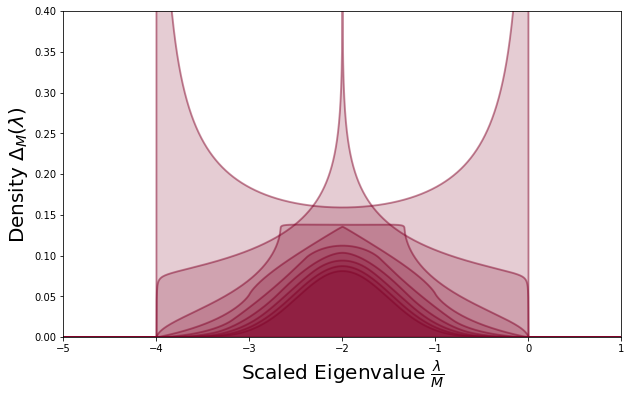
\includegraphics[scale=0.4]{figures/density}
\caption{Eigenvalue distributions $\Delta_M(\lambda)$ of the $M$-dimensional Laplacian}
\label{fig:dos}
\end{figure}
The one dimensional density has two Van Hove singularities at $\lambda=-4,0$
given by the arcsine law $\alpha(\lambda)$, whereas the two dimensional
case has one at $\lambda=-4$ given by the complete elliptic integral
of the first kind $K(m)$. Figure~\ref{fig:dos} reveals that in higher
dimensions singularities do not occur; instead there appear to be
discontinuities in the higher order derivatives. The density smooths out
as repeated convolutions bring it to a normal distrubtion; this is another
way to state the Central Limit Theorem~\cite{}.

In the context of an equation of motion, the laplacian often is scaled by
a diagonal matrix, which may represent anisotropic diffusion. To take this
scaling into account the parameter $D$ is introduced in the arcsine law.
\begin{align}
  \alpha(\lambda|D)=
    \frac{\Pi\left(\frac{\lambda/D+2}{2}\right)}{2\pi D\sqrt{1-\left(\frac{\lambda/D+2}{2}\right)^2}}
  \label{eq:arcsine}
\end{align}
Substituting this limiting density~(\ref{eq:arcsine}) into the second equation
in~(\ref{eq:gamma}) the inverse laplace transform of the powers can be
performed immediately, this time giving non-integer order modified Bessel
functions of the first kind $I_{\frac{l-2}{2}}(4Dt)$, which have the same
asymptotics as in the wigner ensemble case.
\begin{align}
  \Phi(s)=\frac{1}{\sqrt{s}\sqrt{s+8D}}
  \qquad
  \Gamma(t)=2Te^{-4Dt}
  \sum_{l=1}^{\infty}\frac{(\frac{1}{2}-1)!}{(\frac{l}{2}-1)!}\left(\frac{T^2t}{2D}\right)^{\frac{l-2}{2}}
  I_{\frac{l-2}{2}}(4Dt)
\end{align}
\vspace{-20pt}
\begin{align}
  \implies
  \langle \sigma_{\lambda}(t)\rangle
  \asymp
  \sqrt{\frac{D}{T^2}}\mathbb{e}^{\left(\lambda-\frac{T^2}{4D}\right)t}
\end{align}
Since all eigenvalues are negative $\lambda\leq 0$ the moments exponentially
decay to zero, regardless of the values of $T$ and $D$ which is what would be
expected any spectrum with strictly negative eigenvalues.
\begin{figure}[H]
\centering{}
\captionsetup{justification=centering}
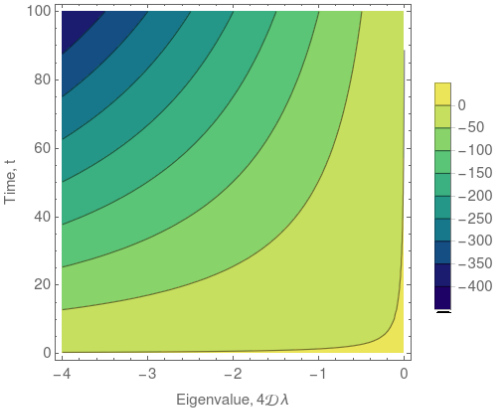
\includegraphics[scale=0.4]{figures/ss1}
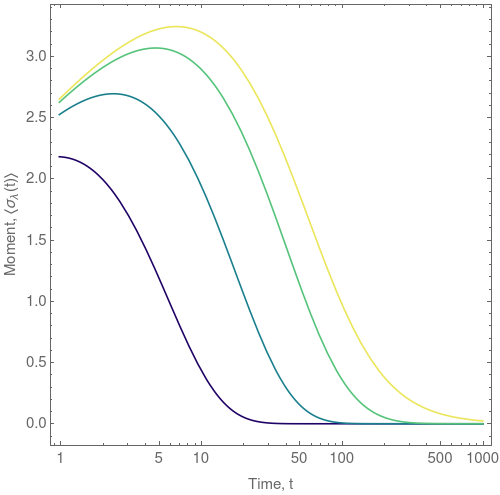
\includegraphics[scale=0.33]{figures/ss}
\caption{Moments $\langle \sigma_{\lambda}(t)\rangle$
in the $\lambda,t$ eigenvalue time plane. The contours are\\ on a log
scale, revealing that all eigenvalue components decay to zero}
\label{fig:ss}
\end{figure}
Analysis on equilibrium values for $\left\langle\sigma_\lambda\right\rangle$
and extraction of timescale $\tau$ like in previous section would go here...
\subsection{Wigner Laplacian Matrices}
A Wigner Laplacian is defined as the sum of a Wigner matrix
of scaling $J$ and an $M$-dimensional laplacian of isotropic scaling $D$.
In the formalism of Free Probability it is possible to express the
$N\rightarrow\infty$ limiting eigenvalue density $\rho$ of a sum of
matrices as the free convolution $\boxplus$ the individual limiting
compact densities $\cap(\lambda|J)$ and $\mu(\lambda|D)$~\cite{Novak2012}.
\begin{align}
  \rho(\lambda|J,D)=\cap(\lambda|J)\boxplus\mu(\lambda|D)
  \label{eq:freeconv}
\end{align}
Unfortunately the general definition of this operation is rather implicit.
The expression can be unpacked in terms of an infinum~\cite{Biane_1997}
and regular convolution $*$ for the specific case of free convolution of
semicircle distrubtion $\cap(\lambda|J)$.
\begin{align}
  \rho(\lambda|J,D)=
  \frac{1}{\pi J^2}
  \inf_{\rho\in[0,\infty)}
  \left\{
  \varepsilon(\lambda,\rho|J,D)
  \geq0
  \right\}\qquad\qquad\quad\\
  \varepsilon(\lambda,\rho|J,D)=
  1-J^2\mu(\lambda|D)*\gamma(\lambda,\rho)
  \qquad\text{where}\quad\gamma(\lambda,\rho)=\frac{1}{\lambda^2+\rho^2}
  \label{eq:inf}
\end{align}
Substituting the distribution $\mu(\lambda|D)$ for the $M$-dimensional laplacian
\eqref{eq:mlap} with isotropic diffusion $D$ yields an expression for the contours
$\varepsilon(\lambda,\rho|J,D)$ as the repeated convolution of arcsine laws
~\eqref{eq:arcsine} with $\gamma(\lambda,\rho)$. Numerically this is efficiently
evaluated in the fourier domain.
\begin{figure}[H]
\centering{}
\captionsetup{justification=centering}
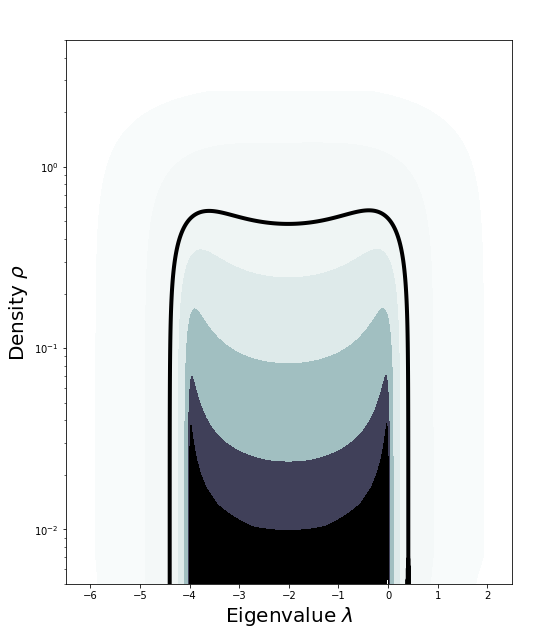
\includegraphics[scale=0.3]{figures/1dinf}
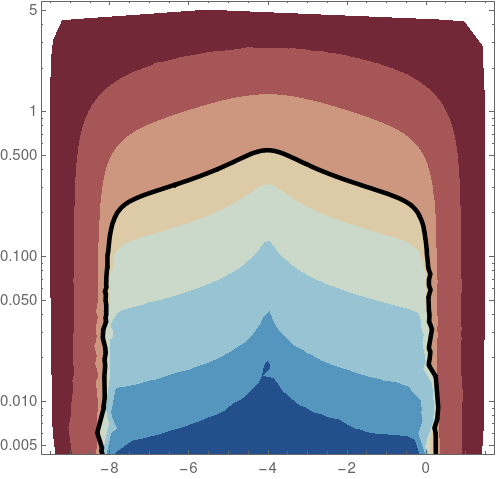
\includegraphics[scale=0.3]{figures/2dinf}
\caption{Left/Right: Numerical evaluation of the contours
$\varepsilon(\lambda,\rho|J,D)$ for the one/two dimensional laplacian. The
infinum picks out the contour at the value zero shown as a black line
for given values of $J,D=1$}
\label{fig:inf}
\end{figure}
The infinum minimises the value of the contour function $\varepsilon(\lambda,\rho|J,D)$
in the domain $\rho\in[0,\infty)$ and $\varepsilon\geq0$ and thus picks out the contour
at $\varepsilon(\lambda,\rho|J,D)=0$. This becomes a transcendental equation for
$\rho$, which can be expressed as a single integral containing the fourier transfrom of
$\gamma(\lambda,\rho)$ and the $M$-th power of the zeroth order Bessel function of the first
kind $J_0(k)$.
\begin{align}
        \int_{-\infty}^{\infty}\!
          \left(J_0(k)\mathbb{e}^{\mathbb{i}k}\right)^M
          \mathbb{e}^{\frac{\mathbb{i}k\lambda-|k|\rho}{2D}}
        \,\mathrm{d}k
    =\frac{2\rho}{J^2}\label{eq:density}
\end{align}
Looking at the functional form of the above equation indicates that different choices
for $J,D$ amount to shifting and scaling such that the infinum picks out neighbouring
contours. Indeed in Figure \ref{fig:inf} an approach to the semicircle and convoluted
arcsine laws can be seen for positive and negative contours respectively.

Figure \ref{fig:spectra} reveals the corresponance between the density given by
the transcendental equation~\eqref{eq:density} and empirical eigenvalue histograms of
Wigner Laplacians. The analytical density had to be renormalised such that its integral
is one. While the shifting of the bounds of the distribution towards negative
eigenvalues matches well, it appears that there is an error in scaling which manifests
as a discrepency at intermediate values of $J$ and $D$ between empirical and theoretical
densities.
\begin{figure}[H]
\centering{}
\captionsetup{justification=centering}
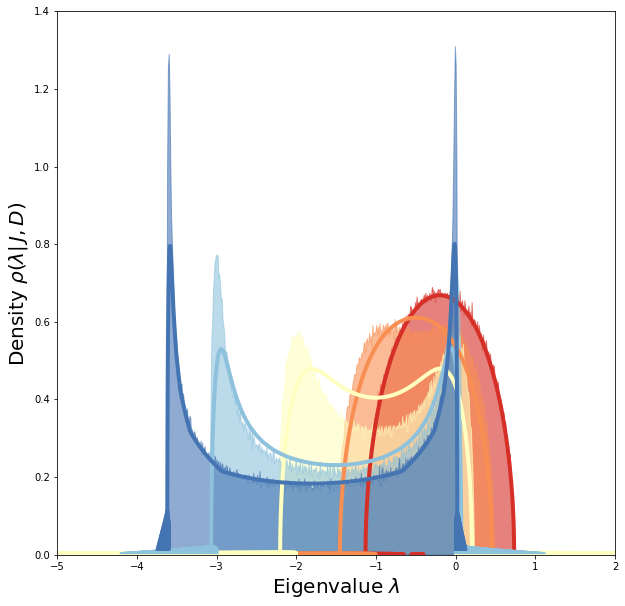
\includegraphics[scale=0.3]{figures/interaction1d}
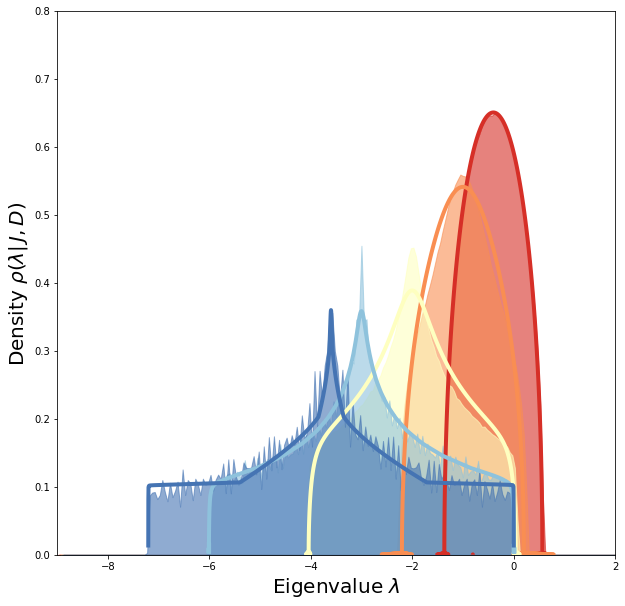
\includegraphics[scale=0.3]{figures/interaction2d}
\caption{Left/Right: Eigenvalue density of one/two dimensional Wigner \\Laplacian
$\rho(\lambda|\,J,D)$ for parameter values $D\in(0,1)$ and $J=1-D$}
\label{fig:spectra}
\end{figure}
Numerical evaluation of integrals in \eqref{eq:gamma} should follow here to
determine moments. Expecting to observe crossover region where equilibrium
is reached in finite time for sufficiently large $D$...

\bibliography{bibliography/biblio}
\bibliographystyle{ieeetr}
\end{document}
